\documentclass{chi2011}
\usepackage{times}
% \usepackage{url}
\usepackage{graphics}
\usepackage{color}
\usepackage[pdftex]{hyperref}
\hypersetup{%
pdftitle={Your Title},
pdfauthor={Your Authors},
pdfkeywords={your keywords},
bookmarksnumbered,
pdfstartview={FitH},
colorlinks,
citecolor=black,
filecolor=black,
linkcolor=black,
urlcolor=black,
breaklinks=true,
}
\newcommand{\comment}[1]{}
\definecolor{Orange}{rgb}{1,0.5,0}
\definecolor{grey}{rgb}{0.6,0.6,0.6}
\newcommand{\todo}[1]{\textsf{\textbf{\textcolor{Orange}{[[#1]]}}}}

\pagenumbering{arabic}  % Arabic page numbers for submission.  Remove this line to eliminate page numbers for the camera ready copy

\begin{document}
% To make various LaTeX processors do the right thing with page size.
\special{papersize=8.5in,11in}
\setlength{\paperheight}{11in}
\setlength{\paperwidth}{8.5in}
\setlength{\pdfpageheight}{\paperheight}
\setlength{\pdfpagewidth}{\paperwidth}

% Use this command to override the default ACM copyright statement
% (e.g. for preprints). Remove for camera ready copy.
\toappear{Submitted for review to CHI 2011.}

\title{Text input mechanisms for devices with backside touch input}
\numberofauthors{2}
\author{
  \alignauthor Author 1\\
    \affaddr{Affiliation}\\
    \affaddr{Affiliation}\\
    \email{author@a.com}
  \alignauthor Author 2\\
    \affaddr{Affiliation}\\
    \affaddr{Affiliation}\\
    \email{author2@b.com}
}

\maketitle

\begin{abstract}
  Talk about text input being a problem for foot-scale devices. The paper explains a few mechanisms that would mitigate that. Discusses the exeperiment gains, results both qualitative and quantitative.
\end{abstract}

\keywords{QWERTY, multitouch, touchscreens, keystroke per character(KSPC), words per minute(WPM)} 

\category{H.5.2}{Interaction techniques and devices}{Miscellaneous}[Optional sub-category]


\section{Introduction}

With the recent rise in sales in the smartphone/PDA market
and the recent launch of several tablet form-factor devices (Tablet PCs, Apple iPad, Amazon's Kindle), users increasingly use medium sized touch screens. These screens offer
more screen space than a traditional phone, and can arguably be more
effective in text-input tasks. Due to increased size and weight,
however, these devices require specific postures for the users to be
able to input text. Therefore, text entry on such devices continues to be a difficult problem.

As mentioned above, the tablet form-factor introduces two major problems for the user. 

Firstly, the larger form-factor makes it hard to type while not seated. Since a tablet is portable, it is an ideal device for use while mobile. By this we mean situations when the user is actually moving between different places, but mostly stationary. Commuters standing in a train are a good example of users who would benefit from using a computing device while standing, walking or sitting and briefly holding their device.
\begin{figure}
    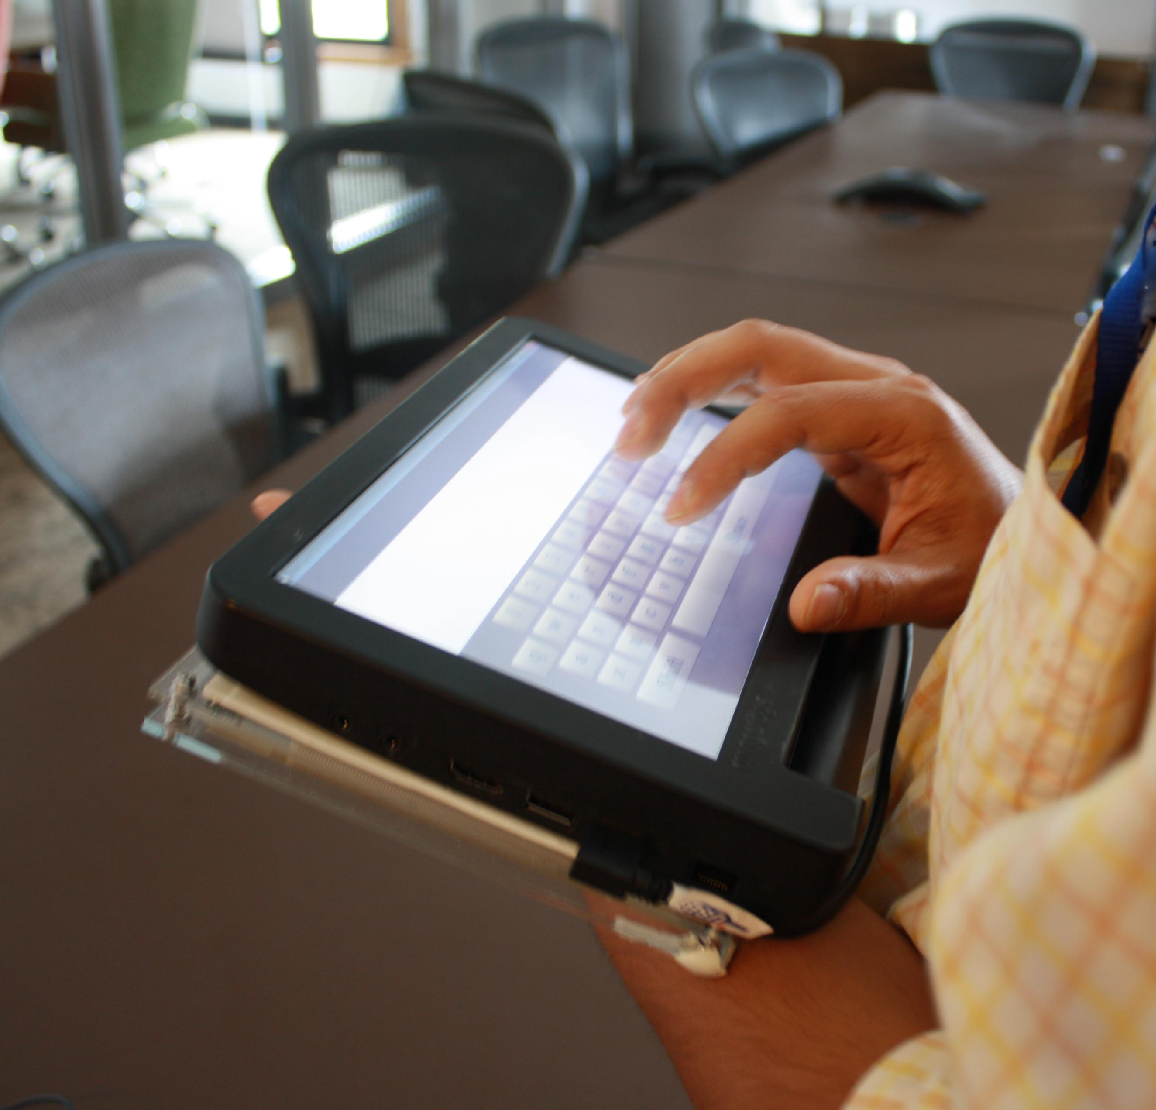
\includegraphics[scale=0.35]{Figures/device_hold.pdf} 
  	\caption{A user holding a tablet form-factor device and trying to enter text. It can be seen how this is unstable and unnatural.}
    \label{fig:device_hold}
\end{figure}
Unlike a mobile phone, however, a larger (e.g. 7+ inches wide)  keyboard (soft or otherwise) does not work well with two thumbs because of the relatively large distance that the thumbs must travel to reach the appropriate keys. The weight of the device compounds the problem of typing by straining the hands to support the device while making precise movements to position the thumbs over the proper keys. While standing, many users resort to a different pose, in which one arm supports the device while the other hand types with a single finger (Figure~\ref{fig:device_hold}). 

The second problem with tablet form-factor is that direct touch or pen input cause the issue of occlusion. Previous work suggests that such scenarios involve contortions of fingers and hands to achieve a configuration that allows for reading the screen while entering text. \cite{Vogel}

At the same time, there has recently been a push in the industry for devices with "backside" input, in which the device has a touch input device or keyboard on the opposite side of the main display. Notion Ink's Adam PC has a backside trackpad [1]. Samsung, Toshiba and Sony have also been making effort towards backside touch input \todo{citations}. As manufacturers start to include backside input in their devices, we have an opportunity to take advantage of this new input modality to improve the users speed, accuracy and comfort while entering text on their tablet form-factor devices. A "natural" method of holding such a device is to have hands on both the sides with fingers wrapped around on the back. \cite{Vogel} (Figure~\ref{fig:natural})

We believe that back-of-device interactions offer solution to both the problems mentioned above because the fingers naturally rest on the back of the device while holding it, thereby relieving the common problem of trying to hold a device with one hand while tapping with the other. (Figure~\ref{fig:device_hold}) Moreover, keeping the finger input on the back keeps the fingers from getting in the way of viewing the information on the screen. A concrete scenario to consider is when the user is mobile but still visually focused, but occasionally losing focus while entering text (for example while commuting on a train).  With a QWERTY keyboard, users have to orient themselves again after each lapse. Such scenarios can benefit from mechanisms that don't require the user to reorient themselves when they lose focus.  Scenarios in which the user is only intermittently focused, such as when they are walking, require mechanisms that help the user memorize certain set patterns and configurations of fingers, that they could later replicate even without looking at the interface. 

In this paper we present two text-input mechanisms that can be tested on devices with back-of-device touch input. The goal is to provide mechanisms that could allow users to enter text on devices with tablet form-factor and back-of-device touch input in a way that eliminates the problems of occlusion of screen space inherent to touch and pen input, and uses the established effectiveness of vertical movements on back-of-device touch input \cite{Wobbrock} by giving freedom of movement to multiple fingers. Previous studies \cite{RearType},\cite{LucidTouch} have tried to investigate a similar design space, but there is lack of systematic understanding of back-of-device text-input in the absence of additional hardware like hover sensing (LucidTouch) and discrete physical keys (RearType). 

In this paper we present a novel text-input mechanism that could be
tested on devices with back-of-device touch input, and examine QWERTY
layouts on both the front and back of the device for comparison. The
goal is to provide mechanisms that could allow users to enter text on
devices with larger screens and back-of-device touch input in a way
that eliminates the problems of occlusion of screen space inherent to
touch and pen input, and uses the established effectiveness of
vertical movements on back-of-device touch input \todo{cite Wobbrock}
by giving freedom of movement to multiple fingers.  Our work stands in
contrast to other recent work which requires additional hardware, such
as hover sensing \todo{cite LucidTouch} or discreet physical keys
\cite{RearType}.

We have designed a chording-based touch input mechanism specifically for devices with a back-of-device touch input.  This mechanism shows promise in the scenarios described above.  Figure~\ref{fig:natural} illustrates that entering text on the back of the device results in a more natural, comfortable and stable pose than the commonly adopted pose shown in Figure~\ref{fig:device_hold}.  We designed the mechanism to use large, relatively inaccurate finger movements as the building
block for chords.  This allows the user to exploit proprioceptive feedback (e.g. the feedback from in the nervous system of the hands that signals the relative positions of the fingers to one another) to
increase their speed and accuracy by reducing or eliminating the visual feedback required to enter text. We also designed a backside-QWERTY mechanism that allows users to use multiple fingers to manipulate multiple cursors, thereby entering text. Details on both the mechanisms can be found later in the paper.

\begin{figure*}
    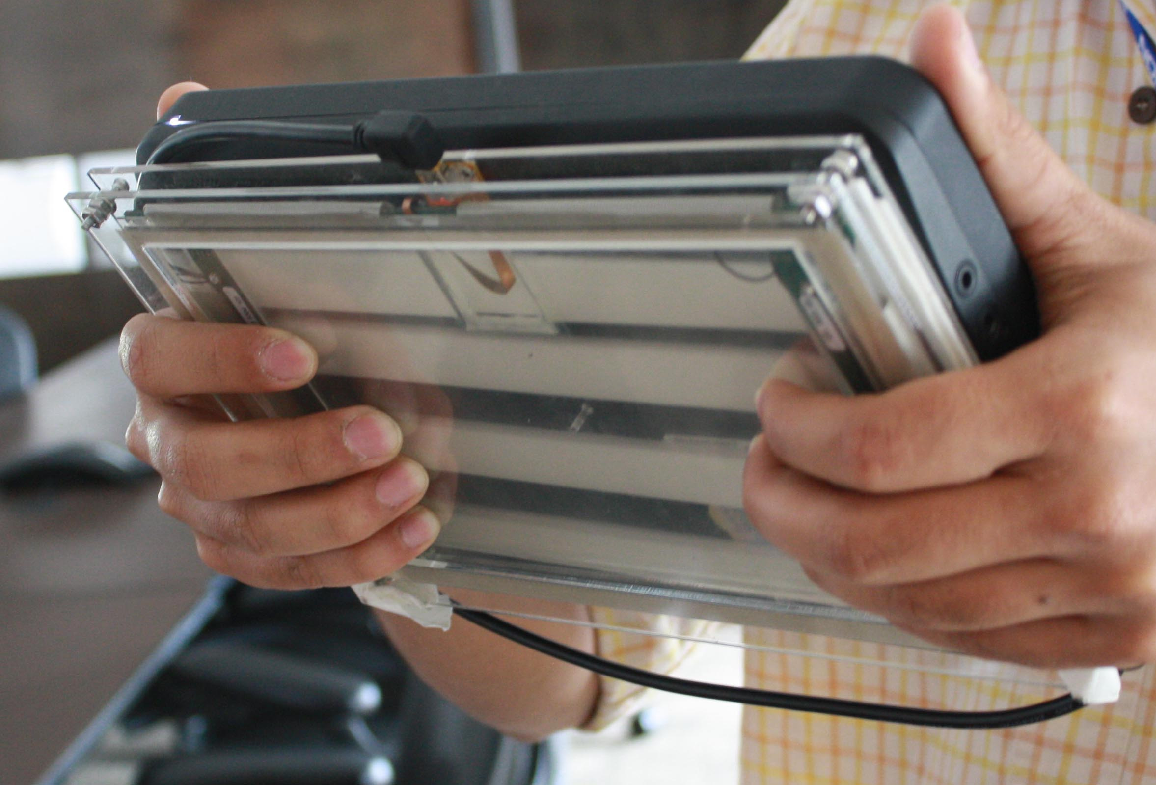
\includegraphics[scale=0.43]{Figures/natural1.pdf} 
     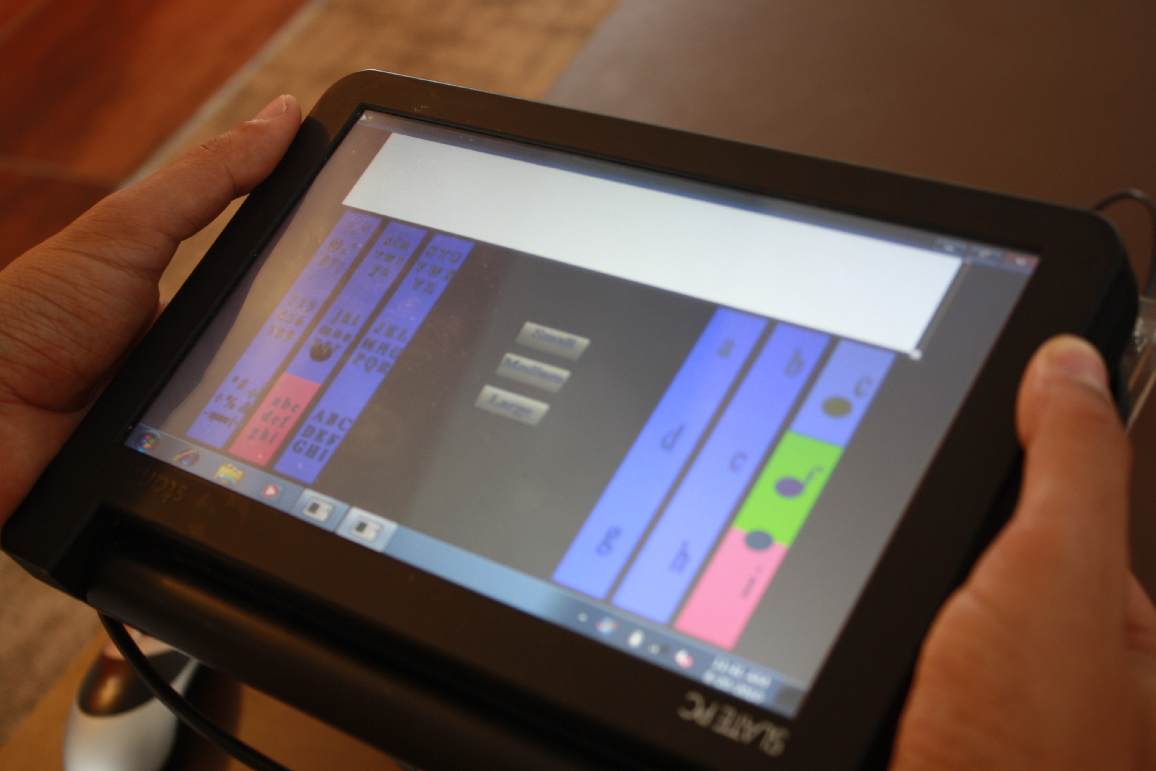
\includegraphics[scale=0.43]{Figures/natural2.pdf} 
     \caption{A user holding a mobile device with medium-sized touch
       screen in a natural and stable posture. The user is able to see
       his finger positions on the screen on the front. The figure
       also shows our hardware prototype with a multitouch screen on
       the rear of a Slate PC.}
        \label{fig:natural}
\end{figure*}

In the paper we detail our initial quantitative and qualitative investigation of these new mechanisms. However, just like in the case of other exploratory works \cite{RearType} our focus for this phase of experimentation was to determine if users find such input mechanisms usable or frustrating. There can also be additional concerns with use of back-of-device touch input, like minimized grip stability. In view of such issues it was necessary to investigate the user perception around back-of-device text-input. To capture that we use the NASA Task Load Index (TLX) and present an analysis of the reported user experience. Using a hardware prototype with a multitouch input on both the back and the front of the device, we compare the performance of the novel chording mechanism and a backside QWERTY with a standard soft QWERTY keyboard on the front or the back of the device in a controlled, 36-user study. We found that with less than an hour of training, users of the backside-QWERTY were able to type 3/4th as fast as soft-QWERTY. Also the chording mechanism turned out to be the most efficient in terms of KSPC (Keystrokes per Character)

\section{Related Work}

Some recent efforts have investigated alternate methods of text inputs. Some of them like BlindType \cite{BlindType} (also \cite{Brewster}) try to let the user type without doing visual search, and by doing ambiguity resolution and error correction. Some other efforts like SWYPE investigate approaches more disconnected from traditional keypads. SWYPE \cite{Swype} is a mechanism that allows users to draw spellings on the keypad, instead of pressing individual keys. However, all of these are for devices that are small scale and are meant for front-side touch input.  As such, they do not address the issue of user pose.

The Grippity keyboard \cite{Grippity} allows users to type on the back, using a QWERTY layout. The interface is see through, so that the users can naturally know the key that they are trying to press. However, Grippity is supposed to be a peripheral device and act as a wireless keyboard. This need not necessarily be of value in the scenarios we mentioned above. The RearType keyboard goes a step further, in providing a familiar layout of physical keys on the back of a device for text entry. This leads to less occlusion and clutter on the paired front screen. The results for RearType also look promising \cite{RearType}. However, in spite of all the advantages that it offers, RearType requires additional hardware in terms of physical keys on the back of the device. Moreover, it uses the space on the back of the device to just enable text-input, whereas devices that have back-of-device touch input, use it for multiple scenarios, as in the case of LucidTouch \cite{LucidTouch}. LucidTouch uses touch+hover sensing to determine finger positions at the back of the device. This is then used to create the experience of semitransparency to gain greater accuracy in terms of approaching targets. Both LucidTouch and RearType require additional hardware, and are not designed to work for devices with back-of-device touch input. The fact that there does and will continue to exist hardware (with back-of-device touch input) which does not include these additional hardware capability implies that techniques which do not rely on it will be needed.

Wearable computing users often use one-handed chording keyboards, such as the Ekatetra \cite{Ekatetra} or the Twiddler \cite{Twiddler}, as their text input mechanism. One handed chording keyboards are almost as old as computers themselves, with Doug Englebart demonstrating one in 1968 after many years of work \cite{Englebart}. Chording can be used to free up a hand for, e.g. supporting a device.  Unfortunately, this requires a secondary device for the user, if a standard chording keyboard is to be used.  Peripherals are problematic because they get lost or are often stuffed away deeply in a bag, making them inconvenient for spontaneous use. However, there is prior work that suggests that chording mechanisms hold potential, sometimes even more than traditional keyboards \cite{Conrad}. There is also work on optimal mappings of chords to characters \cite{Gopher}, which can act as inspiration for future experimentation. 

With training, chording keyboards, in conjunction with phonetic encoding of words can be used to dramatically improve the speed of text entry.  Stenotype keyboards, used by court transcriptionists and closed captioners, allow for transciption speeds in excess of 300 words per minute (WPM) for some (well trained) users.  For reference, one study found that average users type at 33 WPM for transcription and 19 WPM for composition \cite{Karat}.

In addition to this, researchers have also explored use of multitouch screens for text input. Shin et al \cite{Shin} implemented a multi-point touch input mechanism and compared it against a single point touch. Moreover, Schmidt et al \cite{Schmidt} have investigated multitouch text input on tabletop displays. Others like Mackenzie have tried to analyze the effectiveness of various different mechanisms and layouts on soft keyboards \cite{Mac}. However, none of these systems have tried to investigate the use of multiple touches on the back of a device while holding the device in a more stable posture.


\section{Scenarios}

We envisioned some scenarios where people might need alternative text
input mechanisms. For each scenario, we then proposed a possible
mechanism that could be helpful in entering text with accuracy, and
reasonable speed. It should be noted that the theme of research was
not to necessarily outrun soft QWERTY in terms of speed, but to
propose mechanisms that could work with reasonable performance in
scenarios listed.

\subsection{Stationary and visually focused}

This is the best case scenario, and also the one that soft-QWERTY
keyboard is perfectly suited for. In this scenario, the user is
stationary (not walking or moving) and can adjust to reach an optimal
configuration. This includes resting the device on the lap, and
entering text similar to an actual keyboard.

\subsection{Mobile and visually focused}

This is the case where the user is moving but has enough time to do
operations that require visual focus on the screen. This includes
scenarios like commuting (standing or sitting). The challenge here is
that due to occasional loss of focus while entering the text, users
have to orient themselves again after each lapse. Such scenarios would
require mechanisms that don't necessarily require the used to
re-orient themselves time and again. In short, mechanisms designed for
such scenarios would allow the user to constantly touch the screen and
still be able to signal input, as and when required.

\subsection{Mobile and intermittently focused}

This is the worst case scenario, and it occurs in cases when the user
is otherwise involved in some activity, but still has a need to enter
text. This includes walking, when the user is actually focused on the
path and is entering text on the side. Being able to enter text in
this scenario, on devices of larger form factor is a challenge. Such
scenarios would require mechanisms that have unique formations or
representations that the user can memorize over time. This also means
that the mechanisms would reduce the amount of visual search that the
user has to perform, in order to enter a particular character.
 


\section{Experiment}
\subsection{Participants}

For the purpose of the study we tried to keep the backgrounds of the
participants mixed, but also ensured that all of them have decent
exposure to typing on QWERTY keyboards (not necessarily
soft-QWERTY). The participants in the study were all working
professionals with more than 3 years of experience (on an average)
with QWERTY keyboards. According to post-test interviews, out of the
total of 36 participants in the study, 32 participants had prior
experience with soft-QWERTY keyboards. This information was important
as familiarity with a particular style of text-input mechanism gets
reflected in the kind of speed people achieve with the same. Though we
tried to achieve a reasonable mix of backgrounds for participants, we
acknowledge the fact that we still had a sample that was
experienced. Therefore, our results are representative of participants
who have had reasonable level of exposure to typing on QWERTY
keyboards. For novices, the results might be different, in any
direction.

\subsection{Phase 1: Usability test}

After we implemented the QWERTY, backside QWERTY and chording
mechanism, we conducted two rounds of usability evaluation. The first
one with 3 participants, and the second one with 6 participants. For
the purpose of the usability study we picked a text corpus that was
different from the corpus used in the phase 2. Both the corpora were
generated by choosing randomly from Scott Mackenzie's text corpus
[Reference], and were mutually exclusive. The statistics for the two
are listed in Table 1.

\begin{table*}
	\centering
		\begin{tabular}{|l|c|c|} \hline
		                         & Experiment corpus & Usability test corpus \\ \hline
			 Average phrase length & 15.07 & 15.67 \\ \hline
			 Number of words & 76 & 81 \\ \hline
			 Unique words & 62 & 67 \\ \hline
			 Min. length of word & 1 & 1 \\ \hline
			 Max. length of word & 11 & 12 \\ \hline
			 Average word length & 4.95 & 4.43 \\ \hline
			 Number of characters & 437 & 425 \\ \hline
			 Correlation with English & 0.9297 & 0.9377 \\ \hline
		\end{tabular}
	\caption{Statistics for text corpora}
	\label{tab:StatisticsForTextCorpora}
\end{table*}

The participants in the usability test spent 20 minutes familiarizing
themselves with the interface and were then asked to enter the entire
usability test corpus. The entire process was captured on videos and
post-test interviews were also conducted. Based on the post-test
interviews and analysis of videos, changes to the interfaces were
made.

\subsection{Phase 2: Scientific experiment}
\subsubsection{Conditions}

The experiment had three conditions. As mentioned earlier, there were
a total of 36 participants. Each condition had 12 participants. The
three conditions were:

\begin{itemize}
	\item QWERTY
	\item Backside QWERTY
	\item Chording Mechanism
\end{itemize}
\subsubsection{Data collection methods}

To make sure that all the important aspects of the experiment and the
feedback from the users is captured fully, we used multiple data
collection methods:

\begin{itemize}
\item Videos: All the sessions were fully recorded. In total, around
  20 hours of videos were recorded, by the end of the experiment.
\item Data Logs: All the mechanisms had a built in data logging
  feature, that recorded each and every action of the user, along with
  timestamps. This helped in understanding parts of the videos, where
  the user was stuck or had trouble accomplishing what they wanted.
\item Post-session interviews: After each session, the participants
  were asked to report on their experience with the interface. To give
  the discussion some structure, the users were asked the following
  questions:

\begin{enumerate}
	\item What did you like the most?
	\item What did you dislike the most?
	\item What would you change in the interface?
\end{enumerate}

\item NASA task load index: To be able to quantitatively capture the
  experience with the interfaces, the NASA task load index was
  used. The NASA Task Load Index (NASA-TLX) is a subjective,
  multidimensional assessment tool that rates perceived workload on
  six different subscales: Mental Demand, Physical Demand, Temporal
  Demand, Performance, Effort, and Frustration. It was developed by
  the Human Performance Group at NASA's Ames Research Center over a
  three year development cycle that included more than 40 laboratory
  simulations [Reference] [Reference]. It has been cited in over 550
  studies[Reference] and a recent search for NASA-TLX on Google
  Scholar revealed over 3,660 articles. These statistics highlight the
  large influence the NASA-TLX has had in Human Factors
  research. Therefore, we chose it as a tool in our experiment to
  capture the user experience.

\end{itemize}
\subsubsection{Measures}
\begin{itemize}
	\item Keystrokes Per Character (KSPC)
	\item Words Per Minute (WPM)
	\item Speed vs Accuracy tradeoff 
\end{itemize}
\subsubsection{Process}

The participants in the study were supposed to go through the
following steps during the study. Care was taken that the steps remain
the same across all participants so as to control the
environment. Ideally, the mechanisms should have been tested out in
the scenarios that we had earlier listed. However, the lack of prior
research on the topic, suggested that the first few research cycles
should be conducted under controlled conditions. This eliminated the
possibility of the environment acting as a confounding variable in the
experiment.

\begin{enumerate}
\item Participants were briefed about the goal of the session. They
  were also briefed about the structure of the session.
\item They were given a brief introduction to the input
  mechanism. This was done by one of the researchers.
\item They were given a the test corpus and asked to spend the next 20
  mins familiarizing themselves with the input mechanism. The text
  they were supposed was the test corpus.
\item The entire process was videotaped for data analysis and
  validation purposes.
\item After 20 minutes, they were handed over the experiment
  corpus. They were asked to input the corpus in its entirety, using
  the mechanism that they had just encountered. They were asked to be
  accurate with their input, and the system would underline their
  mistakes as and when they occur.
\item Once the participants had entered the entire text without any
  errors, they were handed the NASA TLX questionaire and asked to rate
  their experience. Since the index is relative they were asked to
  compare their experience with their previous exposure to a soft
  QWERTY keyboard. This was also done for the QWERTY mechanism, just
  to make sure that the mechanism is a fair representation of the
  soft-QWERTY family. Since the NASA-TLX is a 20 point scale, we asked
  them to assume that QWERTY was at 10 on each scale. This was done so
  that the individual ratings could be studied in details during
  qualitative analysis.
\item Finally, they were interviewed on any other qualitative feedback
  they had on how to make the mechanisms better.
\end{enumerate}
	

\section{System}

\subsection{Hardware implementation}

We created our hardware prototype using a Stantum Slate PC and a Stantum
multitouch panel[Figure 2]. The multitouch panel was fixed on the back
of the Slate PC. This replicated the same setup as a foot-scale device
with a backside touch input, and enabled us to test out the mechanisms
we had implemented.

\subsection{Software architecture}

One of the major functionalities of the interfaces was projecting the
touch points on the backside multitouch panel, onto Slate PC's
screen. To this effect, the software architecture for all the
mechanisms was split into two modules; the eventlogger and the GUI:

\subsubsection{Event logger}

The event logger iss responsible for capturing the events being
generated by the backside multitouch panel. These events are then
redirected to the GUI using a local socket connection. Since the
volume of the events being generated is huge, we had to make
modifications to the message passing routine of the
eventlogger. Instead of redirecting all the events generated on the
panel, we maintain a list of cursors or touch points and update the
cursors every 200 milliseconds. Whenever there is a change in the
position or state of a cursor, we send an update on the socket. This
ensures that the GUI is not flooded with more updates than it can
process.

\subsubsection{GUI}

The UI for the mechanisms was created in actionscript 3.0. The design
for the individual mechanisms will be explained in a following
section, but on a higher level the GUI receives cursor updates on the
local socket. Depending on the type of update, cursor positions were
updated, expired cursors were destroyed and new cursors were
introduced, as and when required.


\section{Mechanisms}

As mentioned earlier, we have implemented two backside touch input based mechanisms and a standard soft-QWERTY keyboard. 

\subsection{Backside QWERTY}
This mechanism uses the standard QWERTY layout, but with a few modifications. In this mechanism, the user places his fingers on the backside screen and it results in a cursor appearing on the front screen at a location that is vertically above the touch point. This way user can move multiple cursors at the same time, using multiple fingers. To input a particular character, the user must select a particular key with the cursor and then touch the front screen anywhere to signal input. Figure 3 shows a user selecting a character on the backside-QWERTY mechanism.

\begin{figure}
    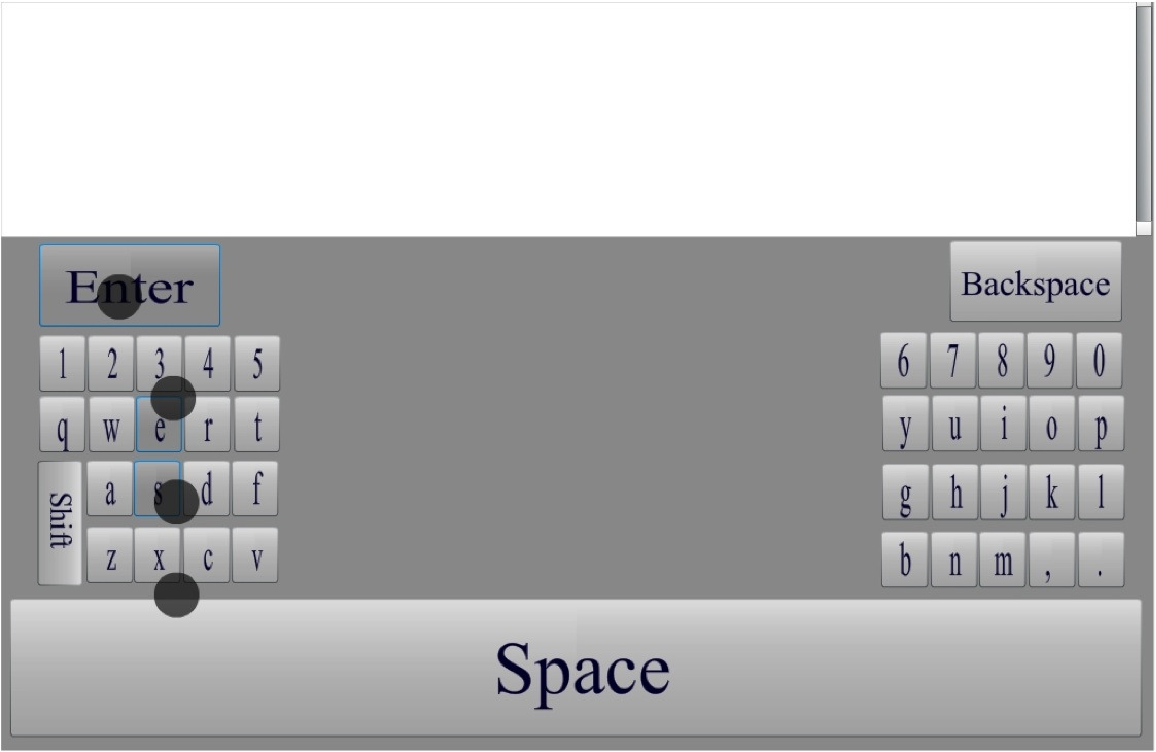
\includegraphics[scale=0.45]{Figures/backside.pdf} 
    \caption{Screenshot of backside-QWERTY with user's fingers on the
      backside screen}
\end{figure}

\subsubsection{Design evolution}

The interface went through two iterations before getting its final shape. The first version used pressure as a method to signal input. When the user increased the pressure on the backside input, a character would be registered.  Unfortunately, pressure input on the Stantum panels appears to be measured by measuring the size of the contact point, rather than actually measuring pressure.  As such, the pressure measurements are inaccurate and difficult to calibrate, especially for the pinky finger. Also, initial tests suggested that being able to control the amount of pressure being applied is hard for users. Since the users were already applying some pressure to drag the cursors around, it turned out to be confusing for them.

Therefore, the second version of the interface accepted a character as input if the user released their finger over that character (also called a "lift-off" at times). However, in this case the chances of giving accidental inputs, by accidentally removing a finger increase manifold. 

As a result we finally shifted to touching (using the thumb) the front panel once the character has been selected, as the method to signal input. This was deliberately done in view of previous research on back-of-device touch input, that advocates the use of thumb-on-front as a complement to fingers on the back techniques. \cite{Wobbrock} 

In the first version we had also modified the keyboard layout to match the finger to key mappings on a QWERTY keyboard, as done by previous research \cite{RearType},\cite{LucidTouch}. However, after the initial test, we realized that users were still doing visual search for keys instead of using their pre-existing motor knowledge of QWERTY. Therefore, a standard QWERTY layout in this case turned out to be more predictable and usable. In hindsight, this is not surprising because previous research \cite{Wobbrock} argued that if finger movement is to be displayed to the user, a "visual-correct" mapping should be used; otherwise a "motor-correct" one may be used. The research on LucidTouch, also indicated that the users were split in terms of their preference for the layout (QWERTY versus inverted-QWERTY). After initial testing, the size of the Space, Backspace and Enter keys was increased to make them easier to select.

\subsection{Chording mechanism}
\begin{figure*}
    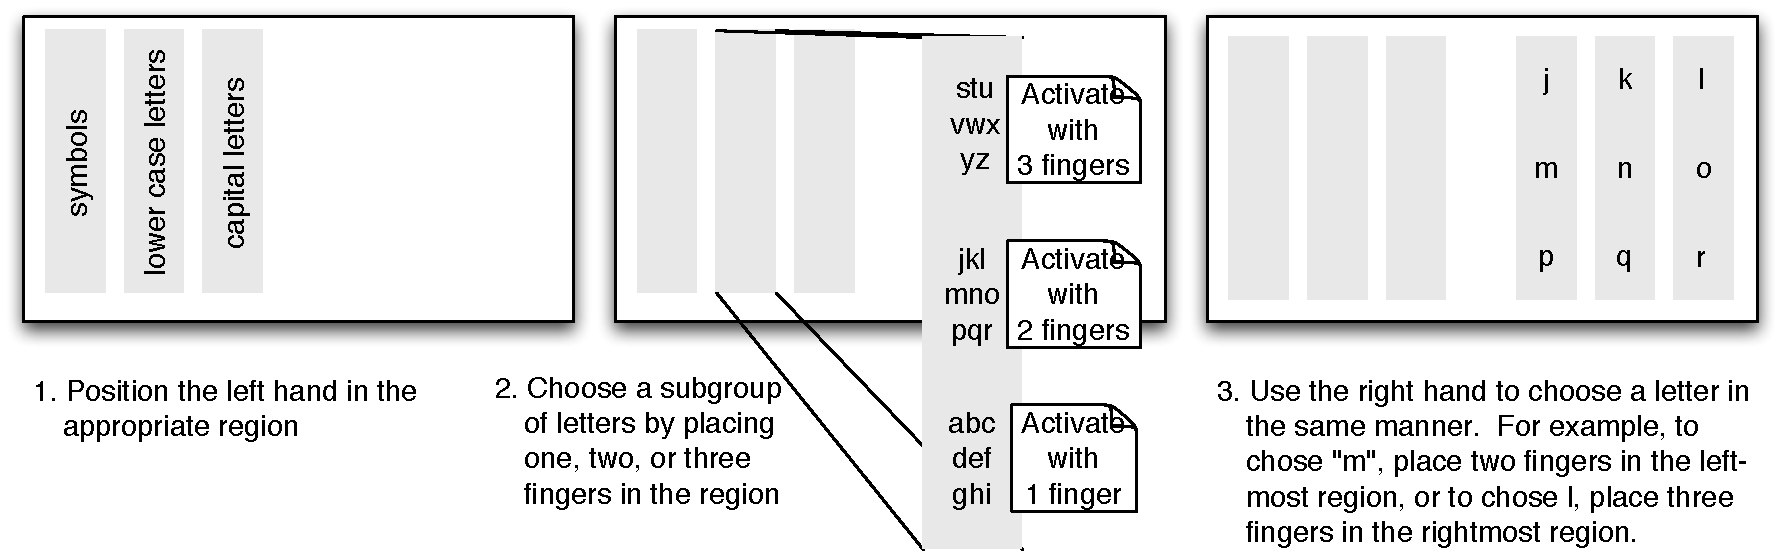
\includegraphics[width=\textwidth]{Figures/chording_explaination.pdf} 
    \caption{Enter the character ``l'' using the chording mechanisms.
      Note that all three steps can be performed simultaneously, for
      proficient users.}
    \label{fig:chording_explanation}
\end{figure*} 

To use the chording mechanism the user extends and contracts their fingers (e.g. move their fingers in the horizontal axis in the natural pose). The user's hand can select three regions, determined exclusively by the distance from the edge of the screen. The movements of the user's left hand select a character class: upper-case, lower-case or symbols. Within these classes, the number of fingers touching the region determines one of three subgroups in the class, with nine characters in each subgroup. The nine characters are broken up into three groups, and the users are supposed to use their right hand to select a character. In summary, the users select a class, a subgroup within a class and a character within the subgroup through each particular configuration of fingers on the back (Figure~\ref{fig:chording_explanation}). It should also be noted that in any given class the user can place one finger to select the lower subgroup, two fingers to select the middle subgroup and three to select the top one.

For example, in Figure~\ref{fig:chording_example} the user places two fingers of the left hand in the middle region to select the class of lower-case letters and the subgroup of "jklmnopqr". The user then places three fingers of the right hand in the rightmost region to select the letter "l".

In our implementation, the number of fingers activating a region is indicated by color changes to the activated regions, in addition to the translucent circles representing the location of the fingers. The user can use these circles to position their fingers in the correct locations. They then touch (using their thumb) anywhere on the front screen to indicate a character input (motivation same as above). Wobbrock et al. \cite{Wobbrock} also talk about the need to minimize vertical movements in back-of-device interactions, which is precisely what our chording mechanism reflects. When the user is learning how to use the chording mechanism, they can enter a character using the step-by-step process described above.  As they become more familiar, however, then can enter chords by touching the device with both hands, in the correct location, simultaneously.

Similar to backside QWERTY and QWERTY, the top quarter of the screen was a scrollable textfield, which displayed the text that was being entered.

The chording mechanism was designed to allow the user to exploit their proprioception (the sense of the relative positions of one's body) rather than tactile feedback, in order to form and exploit kinesthetic memory (short-feedback memory in the nervous system that bypasses cognitive processing for repetitive tasks, often called ``muscle-memory''). Since gross motor movements provide better proprioception, the mechanism was designed to reduce requirements for precise movement.


\begin{figure}
    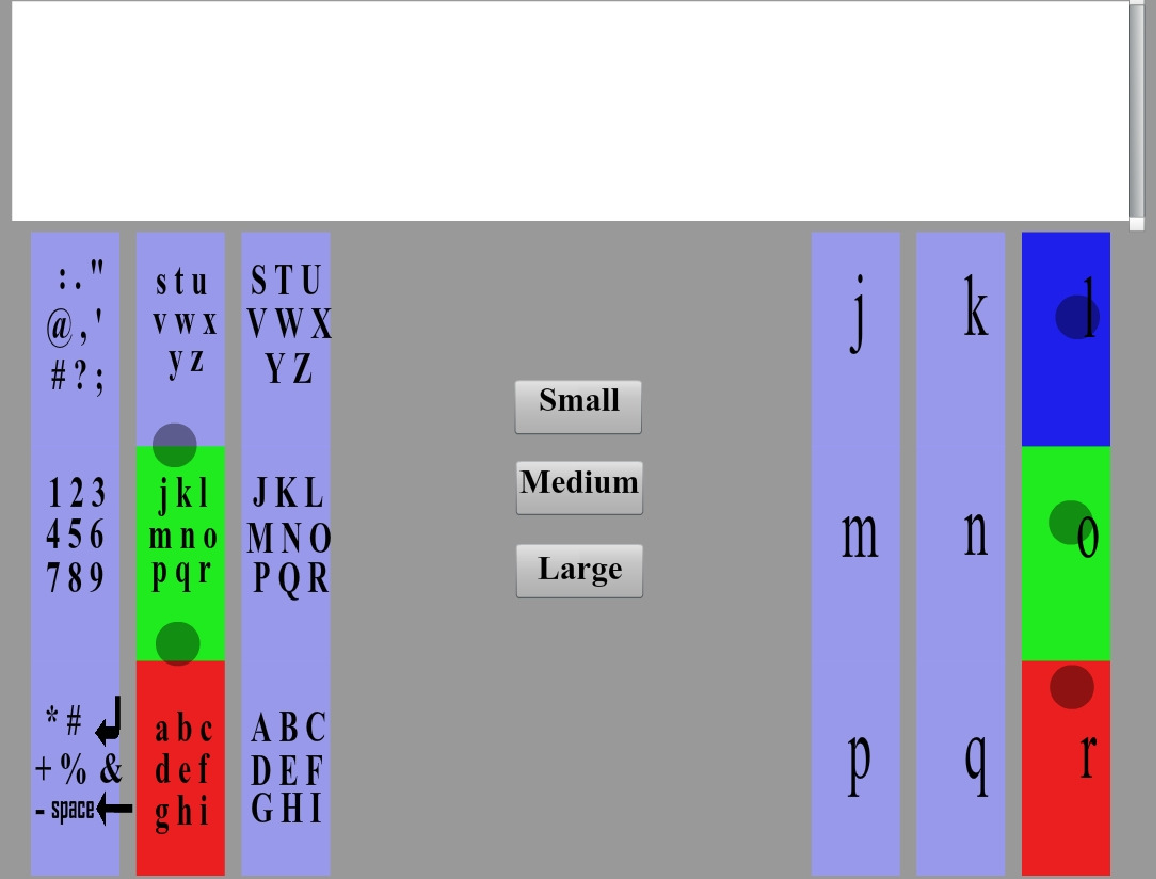
\includegraphics[scale=0.45]{Figures/chording.pdf} 
    \caption{Screenshot of chording mechanism with user's fingers on
      the backside screen trying to form a chord.}
       \label{fig:chording_example}
\end{figure} 
\subsubsection{Design Evolution}

Initial testing suggested that the finger sizes and areas in which users can move comfortably vary a lot. Therefore, in the final version the users were allowed to select from large/medium/small setting, that determined the width of the zones. Users, who had smaller reach, could use these settings to optimize the area of movement. The rest of the design changes pertained to the device itself (like pressure), and therefore the fixes were the same as backside-QWERTY.

\subsection{QWERTY}

This is a standard soft QWERTY keyboard, with no special modifications. The keyboard supports multitouch, which means the users can select the next character to be entered without releasing the currently selected one. The keys turns blue on click, so that the user gets appropriate feedback. The top quarter of the screen is a scrollable textfield, which displays the text that is being entered.



\section{Results}
\subsection{Quantitative results}

We will discuss our quantitative results in terms of the three
measures that we have proposed earlier in the paper.

\subsubsection{Keystrokes Per Character (KSPC)}

KSPC is generally treated as a measure of accuracy, because it
represents the number of keystrokes executed per character. From our
experiment, it turned out that all the three mechanisms were similar
in terms of KSPC measurements as shown in
Figure~\ref{fig:kspc_and_wpm}.

\begin{figure}
    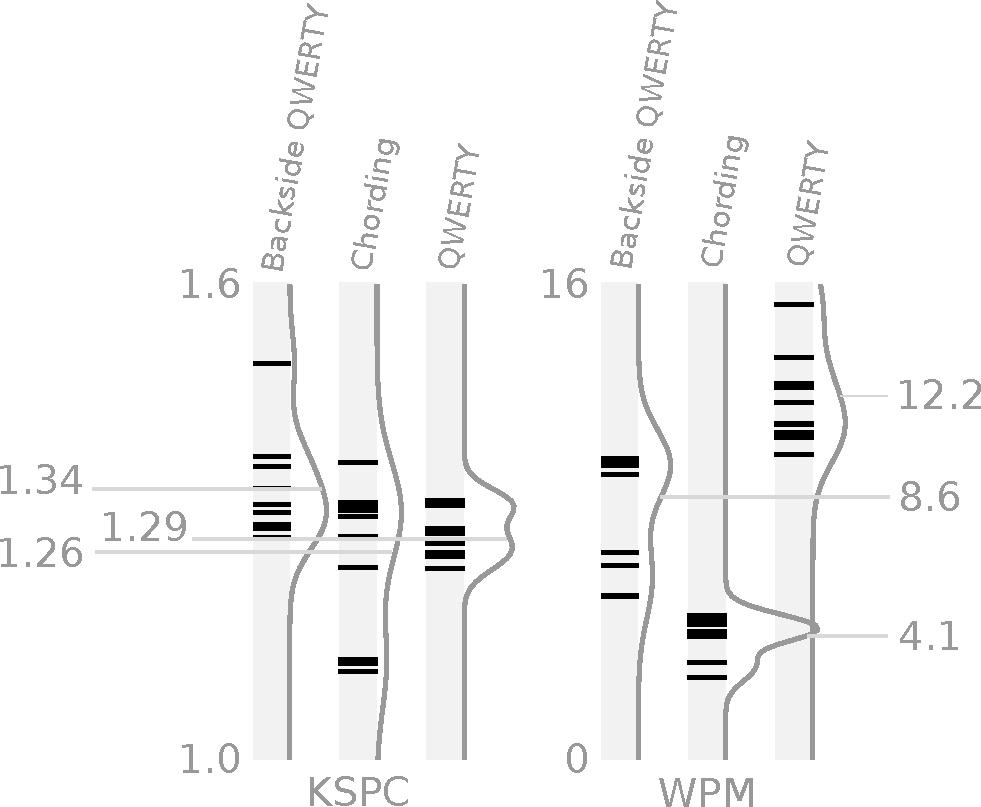
\includegraphics[width=0.5\textwidth]{Figures/kspc_and_wpm.pdf} 
    \caption{Keystrokes-per-character (KSPC) and words-per-minute (WPM) for each mechanism, with means noted.}
    \label{fig:kspc_and_wpm}
\end{figure}

The Chording mechanism was on an average faster than the other two
mechanisms, with the Backside QWERTY being the slowest in terms of
average. However, when we did a t-test between KSPC measurements for
QWERTY and chording mechanism, the p-value turned out to be 0.35. This
suggests that over the test subjects there was no significant
difference between the accuracies of the QWERTY and the chording
mechanisms. Similarly, a t-test between KSPC measurements for QWERTY
and backside QWERTY resulted in a p-value of 0.24, which still lacks
significance. Therefore, both the backside touch input mechanisms were
as accurate as the QWERTY mechanism.

\subsubsection{Words Per Minute (WPM)}

Words Per Minute (WPM) is a measure that is commonly used to represent
the speed of a text input mechanism. Our experiment findings suggested
that QWERTY was still the fastest mechanism, followed by backside
QWERTY and the slowest was chording. Statistics on WPM measurements
can be found in Figure~~\ref{fig:kspc_and_wpm}.  The results suggested
that QWERTY was faster than both backside QWERTY and chording
mechanisms. However, it should be noted that the test sessions were
generally around 20-30 minutes, and each user only interacted with a
mechanism once. Therefore, the fact that backside QWERTY was on a
average 3/4th as fast as the QWERTY mechanism was encouraging. This
led us to explore the results qualitatively and also in terms of speed
versus accuracy trade-off.

\subsubsection{Speed versus Accuracy Trade-off}

In spite of the discussions above, we should acknowledge that none of
these measures can be studied totally independently, and there was a
possibility that the participants were being more accurate by
sacrificing on speed. However, since speed with a particular input
mechanism is often attributed to the amount of exposure and practice,
we had reasons to believe that the comparison of accuracies was still
fair. However, we still did some Speed vs Accuracy analysis for the
three mechanisms and [Figure] is a plot of the same.

\subsubsection{Sample tests}

Since the amount of exposure that the users received during the
sessions was limited, it was obvious that lack of experience with the
mechanisms is also hampering the speed and accuracy
measurements. Therefore, one of the researchers who was involved in
development of the interface and had reasonable exposure to the
interface went through the test in exactly the same fashion as the
participants. This was done to test the capability of the two new
mechanisms in terms of speed and
accuracy. Table~\ref{tab:StatisticsForTestCorpora} shows the
measurements from the same.

\begin{table}
	\centering
		\begin{tabular}{|l|c|c|c|} \hline
		                         & WPM & KSPC \\ \hline
			 Chording & 7.69 & 1.12 \\ \hline
			 Backside QWERTY & 13.231 & 1.152 \\ \hline
		\end{tabular}
	\caption{Sample Measurements}
	\label{tab:StatisticsForTestCorpora}
\end{table}

It can be seen from the table that with decent amount of exposure to
the interface, both the accuracy and the speed seem to show better
trends. However, these measurements are restricted to an individual
and are highly preliminary. To fully establish our claims, larger and
longer studies would have to be conducted.

\subsection{Qualitative results}

As mentioned earlier, the NASA task load index was used to get
subjective ratings on qualitative aspects of the interfaces. This was
just done for the two new mechanisms that were implemented. This was
done deliberately because the participants were asked to give the
ratings keeping in mind their experience with soft-QWERTY
keyboards. Since all the participants in the study had prior exposure
to soft-QWERTY keyboards, this factor was uniform through the
experiment. In the following few paragraphs we summarize the
high-level trends that were derived from the ratings that the
participants assigned to the backside QWERTY and chording
mechanisms. Figure~\ref{fig:tlx-ratings} presents the ratings given by
the users of all three mechanisms.

\subsubsection{Mental Demand}

By just looking at the ratings on the mental demand of the task on the
NASA-TLX scale, it seemed that the users reported less mental load for
the backside-QWERTY as compared to the chording mechanism. When we
conducted a t-test on the ratings, it turned out to have a p-value of
0.02, which suggests that the difference was significant. It also
means that the backside-QWERTY has significantly less mental load than
the chording mechanism. However, the average for backside-QWERTY was
29.5 and that for chording was 43, which means that on an absolute
scale participants thought that the two mechanisms were not mentally
intensive to work with. The chording mechanism was deemed as harder to
understand because in that case, the users were trying to work with
the number of fingers as a method of input. This setup was new for all
the participants in the study, and this also relates back to the low
speed (in WPM) of text entry on the chording mechanism. The averages
are lower than 50 for both the mechanisms, which denotes that quite a
few participants believed that the mechanisms are simpler to
understand and use than QWERTY. This effect was more well defined for
backside-QWERTY (average of 29.5), as opposed to chording (average of
43).

\subsubsection{Physical Demand}

An analysis of the physical demand ratings on the NASA-TLX suggested
that the participants in general found the chording mechanism to be as
physically challenging than the backside-QWERTY. Looking at the kernel
density plots of the two revealed that the distribution of population
across ratings was very similar in the two interfaces. Also a t-test
on the two sets of ratings resulted in a value of 0.91, which meant
that the difference was not significant. Therefore, it is reasonably
fair to say that the two mechanisms were equally easy or equally hard
to use. However, since the averages of both the sets of ratings were
around 50 (10 on the original scale) it means that none of the
mechanisms were exceptionally hard to use, as opposed to each
other. This also means that the two mechanisms were on an average as
easy to use as the QWERTY mechanism, since the participants were
assuming the QWERTY mechanism to have a rating of 10 (on the 20 point
scale) for all metrics.

\subsubsection{Temporal Demand}

This metric was important in the sense that we wanted to make sure
that the participants do not feel rushed during the task. Our aim was
to reproduce the natural experience of entering text, as far as
possible. Therefore, the low average scores (27.5 for both mechanisms)
suggested that the task was not pushing the participants to an extent
that they start noticing it. There were constraints that we had
specified, but none of them seemed to upset the participants. The fact
that there was no time limit to the task, was helpful in this respect.

\subsubsection{Performance}

The NASA-TLX index ratings for performance suggested that both the
interfaces had good performance. The average performance ratings for
both the interfaces were below 8 (on 20 point scale). It should be
noted that a low rating on this scale means good performance. We also
observed that there were two users who gave the chording mechanism a
higher rating, thereby implying that it did not have good
performance. Both these participants had writing speeds that were lass
than the average. This suggests that these participants were
struggling to get accustomed to the device and the mechanism. Their
speed was suffering as a result of the same. We also looked at the
videos from those sessions, and they corroborated the same claim.

\subsubsection{Effort}

The difference between the sets of ratings for backside-QWERTY and
chording was not significant. The t-test results in a p-value of
0.52. However, studying the kernel density plots (see
Figure~\ref{fig:tlx-ratings} more carefully suggested that the
distribution of the opinion on the amount of effort involved in
working with the backside-QWERTY was bimodal. However, for the
chording it was almost evenly distributed around the average
rating. The videos suggested that some of such cases were because the
backside-QWERTY did not allow for change in size of the keyboard,
people who had fingers longer or shorter than average finger sizes had
a harder time with the mechanism as opposed to other. The chording
mechanism on the other hand, did allow for such changes and therefore
got an even distribution of ratings.

\begin{figure*}
    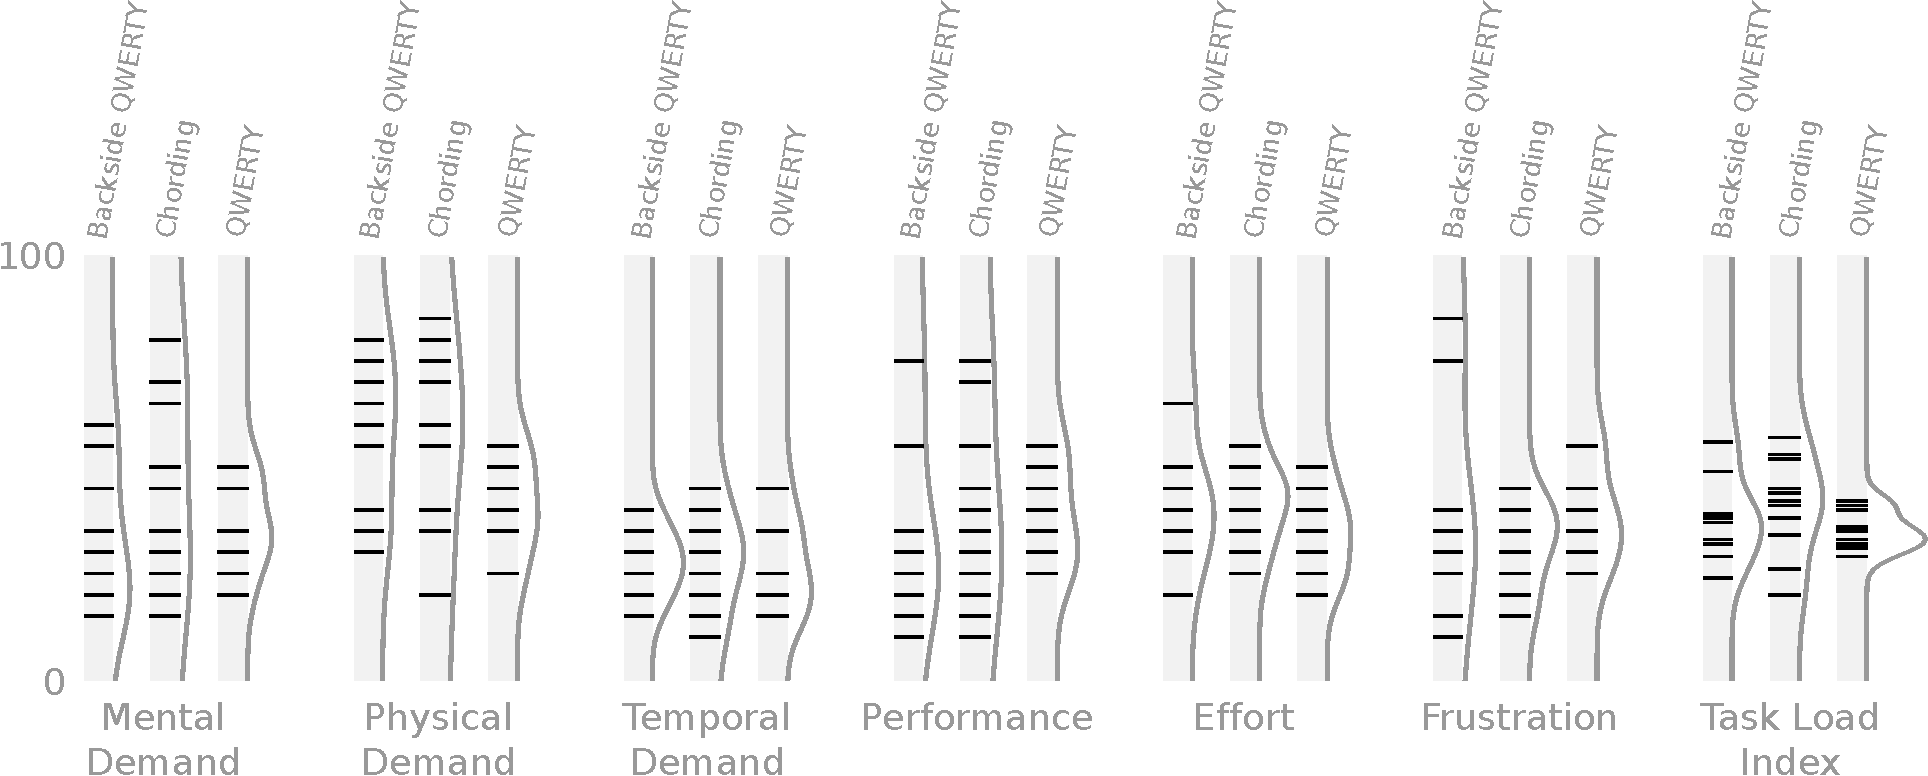
\includegraphics[width=\textwidth]{Figures/hash_and_densities_index.pdf} 
    \caption{NASA-TLX rating for all three input mechanisms}
    \label{fig:tlx-ratings}
\end{figure*}


\subsubsection{Frustration}

The ratings suggested that on an average users were satisfied with the
mechanisms. The frustration levels/ratings were restricted to the
lower half of the scale for chording, however only two users reported
higher levels of frustration with the backside-QWERTY. When we
cross-checked this with our video logs, it turned out that both of
these users had issues with getting accustomed to the mechanisms
primarily because of finger sizes, as pointed out in the last
section. This in turn resulted in the observed frustration on the
NASA-TLX.

\subsubsection{Mean Weighted Scores}
After the individual analysis of the ratings, we used the standardized
methods to calculate the effective weighted task load ratings, as
specified by NASA. Right after filling up the survey, the participants
were also asked to compare metrics against each other. Since there
were 6 metrics (Mental, Physical, Temporal, Performance, Effort,
Frustration), there were $C_{2}^{6}$ possible combinations, and 15
questions in total. After receiving all the responses from the
participants, we found that on an average effective weights for Mental
Demand, Physical Demand, Temporal Demand, Performance, Effort,
Frustration were 4, 3, 3, 1, 2, 2 respectively. In simple words, a
higher weight means that particular dimension or metric has larger
effect towards the load of the task and should be given more weightage
as opposed to others. Initially we thought that interactions with
backside-QWERTY and chording mechanisms were intrinsically different
tasks, and therefore the weights should not be treated as the
same. However, the average weights that were calculated for the two
mechanisms turned out to be very close to each other. This is
understandable from a viewpoint that both the tasks were actually text
entry tasks with same corpus, and same kind of input
method. Therefore, the value that the participants were attaching to
each metric didn't change.

It is apparent from the discussion above, but to clarify again, a low
weighted score on the NASA-TLX means that the overall task load was
low and the experience was pleasant. The backside-QWERTY obtained a
weighted score of 37 on an average, and the chording mechanism got an
average score of 41. The t-test between the two resulted in a p-value
value of 0.22, which means that the difference between the two sets of
effective ratings was not significant. The weighted scores for both
the mechanisms were low, and since the participants were comparing the
mechanisms with their experiences with soft-QWERTY, it can be seen
that the two new mechanisms were definitely welcome by the
participants. From a qualitative standpoint, the mechanisms seemed to
create good user experience, even better than a soft-QWERTY in some
cases.

\subsection{Design guidelines}

After a qualitative and quantitative analysis of our results, we also
did a high-level analysis of our design choices and cross-checked them
against the videos. As a result of this, we came up with some major
design takeaways from this piece of research. Therefore, in this
section we propose some design guidelines for future efforts that look
into text input by utilizing a backside touch input device. These
guidelines are not sufficient, but should definitely be treated as
necessary.

\subsubsection{Movement minimization}

During the study we realized that the amount of movement involved in
selecting a particular character determines the speed that users would
achieve with the mechanism. The post-experiment analysis of usability
test videos corroborated this claim. Once we reduced the size of the
keys and magnified the movement of fingers, the users could cover
larger distances with smaller shifts in position. We also realized
that users are able to control the finger position with very high
accuracy, and therefore these optimizations help them enter text at
higher speeds.

\subsubsection{Multiple finger sizes}

There can be a lot of variation in finger sizes, amongst users. We
accounted for this in the chording mechanism, by having settings that
user could select, if they had fingers larger or shorter than the
average. This was critical for chording mechanism as the users were
trying to form chords at specific locations. For backside-QWERTY, we
did not make this optimization because users were not trying to
position multiple fingers at the same time, and also because in that
case we had tried to optimize between finger movement and key
sizes. Dynamically determining the trade-off between the two,
depending on the finger size would have interfered with the optimal
setting of the system, and influenced other factors.

\subsubsection{Reducing dimensions of movement}

This one is only true for the chording mechanism, but it turned out
from the experiment that a good way to maximize on accuracy is to
reduce the number of dimensions of movement. Traditionally, with a
soft-QWERTY users tend to position themselves in both, x and y
co-ordinate. In the chording mechanism, the y direction was being
controlled by the number of fingers, and therefore the movement was
just restricted to the x direction.

\subsubsection{Visual search vs Recall}

After the usability testing, we also realized that users tend to do a
visual search to find characters instead of recalling from their
previous experiences with QWERTY mechanisms. It turned out the the
layour of keys should be visually intuitive and familiar. As long as
the positions of characters follow a pattern, either pre-existing
(like QWERTY) or familiar (alphabetic), users will be able to accustom
themselves in a few interactions.

\subsubsection{Pressure vs Touch}

As explained earlier, we also experimented with using pressure as a
mode of input, but it turned out that it is hard for users to
accurately control the amount of pressure being applied. This results
in high error rates because of spurious inputs. A design fix that we
used to mitigate the situation was to use touch on the front
screen. Since the two thumbs are anyway used to hold the device, it
was easy for the users to use them to tap on the front screen. This
significantly reduced error rates from the test version to the final
version.

\subsubsection{Touch Cursors}

Both our mechanisms involved showing finger positions on the screen,
and we had to this in a way that we don't hide any information or
don't cause a loss of perception. We achieved this by doing a number
of things. We made the touch cursors transluscent, so that we don't
occlude any information. We also kept the size of the cursor smaller
than the size of an individual key so that they are easier to position
and don't end up selecting multiple keys at the same time.



\section{Future Work}

Since the the speed of the chording mechanism seems to be limited by
its novelty, one important question is ``How can we quickly train
users to use the new mechanism, and maximize their engagement in the
learning process?''  As with other novel input mechanisms, if it is
too difficult for users to learn, they will not use it, even if it
performs much better ( for example, stenographer's text entry
systems).

Future research could also explore haptics and tactile feedback. This
would entail producing vibrations and other cues to signal a change on
the interface. Especially in the case of the chording mechanism,
whenever the user switches from one zone to the other, or selects a
new segment, it could be coupled with some feedback. This would also
help the interface to be used by visually challenged people as well.

The time that the users spent on the mechanisms was limited and short. They had to get accustomed to the interface in around 20 minutes and then start on the test. Future research could be devoted to studying the effects of training times on KSPC and WPM. 

To further minimize the amount of movement in the chording mechanism,
future iterations of the mechanism should use the first touch to
select the zone, and the rest of the touches should select the segment
of the zone, irrespective of position. Therefore, the user won't be
required to try and bring all their fingers into a particular
zone. Instead they would just take one finger to a particular zone and
then place the others at any random location thereby selecting the
segments in the zone that was selected by the first finger. This would
considerably reduce the effort involved in the chording mechanism, and
would also make the interface even less sensitive to positioning.

In the introduction we talked about how there were some scenarios that
we envisioned and observed. However, since this was an exploratory
study we wanted to control as many variables as possible. Therefore,
very similar conditions were reproduced for all the
participants. Future work should test the applications in various
different scenarios, and analyze the appropriateness of different
mechanisms in different scenarios.


\section{Conclusion}
In this paper we proposed two methods of text-input using back-of-device touch input. The methods were developed so that the problem of occlusion due to user's hands could be addressed, and users could enter text in natural postures. A study with 36 participants who had significant exposure to QWERTY keyboards was done to investigate the feasibility of such mechanisms. With less than an hour of training, users of one of the methods were able to type 3/4th as fast as soft-QWERTY. Moreover, an analysis of the perceived workload using the NASA-TLX revealed that there was no significant main effect of input technique on the perceived workload offered by the three mechanisms (soft-QWERTY, backside-QWERTY, chording). In terms of the two back-of-device input mechanisms, backside-QWERTY was found to be faster than chording (WPM), but chording was more accurate (KSPC). Overall the results look promising, but would need further investigation to bring the new mechanisms close (if not at par) with QWERTY typing.

\bibliographystyle{abbrv}
\begin{thebibliography}{1}
\bibitem{1} Adam PC http://notionink.wordpress.com
\bibitem{2} BlinType http://www.blindtype.com
\bibitem{3} SWYPE http://www.swypeinc.com
\bibitem{4} Ekatetra http://www.ekatetra.com
\bibitem{5} Twiddler http://www.handykey.com
\bibitem{6} http://sloan.stanford.edu/mousesite/1968Demo.html
\bibitem{7} Gopher, D., and Raij, D. (1988) "Typing with a two hand chord keyboard - will the QWERTY become obsolete?" IEEE Transactions in System Man and Cybernetics 18, 60l-609. 
\bibitem{8} Shin, H., Lee, W., Lee, G., and Cho, I. 2009. Multi-point touch input method for Korean text entry. In Proceedings of the 27th international Conference Extended Abstracts on Human Factors in Computing Systems (Boston, MA, USA, April 04 - 09, 2009). CHI '09. ACM, New York, NY, 3871-3876.
\bibitem{9} Schmidt T., Konig W., Reiterer H. Text Input on Multitouch Tabletop Displays. EuroVis 2009.
\bibitem{10} Brewster, S.A., Lumsden, J., Bell, M., Hall, M. and Tasker, S. Multimodal 'Eyes-Free' Interaction Techniques for Wear-able Devices. In Proceedings of ACM CHI 2003, ACM Press, Addison-Wesley, 463-480.
\bibitem{11} Cechanowicz, J., Irani, P. and Subramanian, S. Augmenting the Mouse with Pressure Sensitive Input. In Proceedings of ACM CHI 2007, ACM Press, Addison Wesley, 1385-1394.
\bibitem{12} Hoggan, E., Brewster, S.A. and Johnston, J. Investigating the Effectiveness of Tactile Feedback for Mobile Touchscreens. In Proceedings of ACM CHI2008, ACM Press Addison Wesley, 1573-1582.
\bibitem{13} Holleis, P., Huhtala, J. and Häkkilä, J. Studying applications for touch-enabled mobile phone keypads. In Proceedings of TEI 2008, ACM Press,15-18.
\bibitem{14} Mackenzie, I.S., Zhang, S. and Soukoreff, R.W. Text Entry Using Soft Keyboards. Behaviour and Information Technol-ogy, 1999, 18 (4), 235 - 244.
\bibitem{15} MacKenzie, I.S. and Zhang, S.X. An empirical investigation of the novice experience with soft keyboards. Behaviour and Information Technology, 2001, 20 (6), 411-418.
\bibitem{16} MacKenzie, S. and Soukoreff, W. Phrase Sets for Evaluating Text Entry Techniques. In Extended Abstracts of ACM CHI 2003, ACM Press, 754-755.
\bibitem{17} Mizobuchi, S., Terasaki, S., Keski-Jaskari, T., Nousiainen, J., Ryynanen, M. and Silfverberg, M. Making an impression: force-controlled pen input for handheld devices. In Vol II Proceedings of ACM CHI 2005, ACM Press, 1661-1664.
\bibitem{18} Ramos, G., Boulos, M. and Balakrishnan, R. Pressure Wid-gets. In Proceedings of ACM CHI 2004, ACM Press, Addi-son-Wesley, 487-494.
\bibitem{19} Sears, A., Revis, D., Swatski, J., Crittenden, R. and Shnei-derman, B. Investigating Touchscreen Typing: The Effect of Keyboard Size on Typing Speed. Behaviour and Information Technology, 1993.
\bibitem{20} www.yorku.ca/mack/phrases2.txt
\bibitem{21} Hart, S., and Staveland, L. (1988). Development of NASA-TLX (Task Load Index): Results of empirical and theoretical research. In P. Hancock and N. Meshkati (Eds.), Human mental workload (pp. 139-183). Amsterdam: North Holland.
\bibitem{22} Hart, S. (2006). Nasa-Task Load Index (Nasa-TLX); 20 Years Later. Human Factors and Ergonomics Society Annual Meeting Proceedings, 50, 904-908.
\bibitem{23}
\end{thebibliography}

\end{document}